\PassOptionsToPackage{unicode=true}{hyperref} % options for packages loaded elsewhere
\PassOptionsToPackage{hyphens}{url}
%
\documentclass[10pt,xcolor=table,color={dvipsnames,usenames},ignorenonframetext,usepdftitle=false,french]{beamer}
\setbeamertemplate{caption}[numbered]
\setbeamertemplate{caption label separator}{: }
\setbeamercolor{caption name}{fg=normal text.fg}
\beamertemplatenavigationsymbolsempty
\usepackage{caption}
\captionsetup{skip=0pt,belowskip=0pt}
%\setlength\abovecaptionskip{-15pt}
\usepackage{lmodern}
\usepackage{amssymb,amsmath,mathtools,multirow}
\usepackage{float,hhline}
\usepackage{tikz}
\usepackage[tikz]{bclogo}
\usepackage{mathtools}
\usepackage{ifxetex,ifluatex}
\usepackage{fixltx2e} % provides \textsubscript
\ifnum 0\ifxetex 1\fi\ifluatex 1\fi=0 % if pdftex
  \usepackage[T1]{fontenc}
  \usepackage[utf8]{inputenc}
  \usepackage{textcomp} % provides euro and other symbols
\else % if luatex or xelatex
  \usepackage{unicode-math}
  \defaultfontfeatures{Ligatures=TeX,Scale=MatchLowercase}
\fi
\usetheme[coding=utf8,language=english,
,titlepagelogo=img/SACElogo.jpg
]{TorinoTh}
% use upquote if available, for straight quotes in verbatim environments
\IfFileExists{upquote.sty}{\usepackage{upquote}}{}
% use microtype if available
\IfFileExists{microtype.sty}{%
\usepackage[]{microtype}
\UseMicrotypeSet[protrusion]{basicmath} % disable protrusion for tt fonts
}{}
\IfFileExists{parskip.sty}{%
\usepackage{parskip}
}{% else
\setlength{\parindent}{0pt}
\setlength{\parskip}{6pt plus 2pt minus 1pt}
}
\usepackage{hyperref}
\hypersetup{
            pdftitle={R and JDemetra+ : RJDemetra and rjdqa},
            pdfauthor={Alain Quartier-la-Tente},
            pdfborder={0 0 0},
            breaklinks=true}
\urlstyle{same}  % don't use monospace font for urls
\newif\ifbibliography
\usepackage{color}
\usepackage{fancyvrb}
\newcommand{\VerbBar}{|}
\newcommand{\VERB}{\Verb[commandchars=\\\{\}]}
\DefineVerbatimEnvironment{Highlighting}{Verbatim}{commandchars=\\\{\}}
% Add ',fontsize=\small' for more characters per line
\usepackage{framed}
\definecolor{shadecolor}{RGB}{248,248,248}
\newenvironment{Shaded}{\begin{snugshade}}{\end{snugshade}}
\newcommand{\KeywordTok}[1]{\textcolor[rgb]{0.13,0.29,0.53}{\textbf{#1}}}
\newcommand{\DataTypeTok}[1]{\textcolor[rgb]{0.13,0.29,0.53}{#1}}
\newcommand{\DecValTok}[1]{\textcolor[rgb]{0.00,0.00,0.81}{#1}}
\newcommand{\BaseNTok}[1]{\textcolor[rgb]{0.00,0.00,0.81}{#1}}
\newcommand{\FloatTok}[1]{\textcolor[rgb]{0.00,0.00,0.81}{#1}}
\newcommand{\ConstantTok}[1]{\textcolor[rgb]{0.00,0.00,0.00}{#1}}
\newcommand{\CharTok}[1]{\textcolor[rgb]{0.31,0.60,0.02}{#1}}
\newcommand{\SpecialCharTok}[1]{\textcolor[rgb]{0.00,0.00,0.00}{#1}}
\newcommand{\StringTok}[1]{\textcolor[rgb]{0.31,0.60,0.02}{#1}}
\newcommand{\VerbatimStringTok}[1]{\textcolor[rgb]{0.31,0.60,0.02}{#1}}
\newcommand{\SpecialStringTok}[1]{\textcolor[rgb]{0.31,0.60,0.02}{#1}}
\newcommand{\ImportTok}[1]{#1}
\newcommand{\CommentTok}[1]{\textcolor[rgb]{0.56,0.35,0.01}{\textit{#1}}}
\newcommand{\DocumentationTok}[1]{\textcolor[rgb]{0.56,0.35,0.01}{\textbf{\textit{#1}}}}
\newcommand{\AnnotationTok}[1]{\textcolor[rgb]{0.56,0.35,0.01}{\textbf{\textit{#1}}}}
\newcommand{\CommentVarTok}[1]{\textcolor[rgb]{0.56,0.35,0.01}{\textbf{\textit{#1}}}}
\newcommand{\OtherTok}[1]{\textcolor[rgb]{0.56,0.35,0.01}{#1}}
\newcommand{\FunctionTok}[1]{\textcolor[rgb]{0.00,0.00,0.00}{#1}}
\newcommand{\VariableTok}[1]{\textcolor[rgb]{0.00,0.00,0.00}{#1}}
\newcommand{\ControlFlowTok}[1]{\textcolor[rgb]{0.13,0.29,0.53}{\textbf{#1}}}
\newcommand{\OperatorTok}[1]{\textcolor[rgb]{0.81,0.36,0.00}{\textbf{#1}}}
\newcommand{\BuiltInTok}[1]{#1}
\newcommand{\ExtensionTok}[1]{#1}
\newcommand{\PreprocessorTok}[1]{\textcolor[rgb]{0.56,0.35,0.01}{\textit{#1}}}
\newcommand{\AttributeTok}[1]{\textcolor[rgb]{0.77,0.63,0.00}{#1}}
\newcommand{\RegionMarkerTok}[1]{#1}
\newcommand{\InformationTok}[1]{\textcolor[rgb]{0.56,0.35,0.01}{\textbf{\textit{#1}}}}
\newcommand{\WarningTok}[1]{\textcolor[rgb]{0.56,0.35,0.01}{\textbf{\textit{#1}}}}
\newcommand{\AlertTok}[1]{\textcolor[rgb]{0.94,0.16,0.16}{#1}}
\newcommand{\ErrorTok}[1]{\textcolor[rgb]{0.64,0.00,0.00}{\textbf{#1}}}
\newcommand{\NormalTok}[1]{#1}
\usepackage{graphicx,grffile}
\makeatletter
\def\maxwidth{\ifdim\Gin@nat@width>\linewidth\linewidth\else\Gin@nat@width\fi}
\def\maxheight{\ifdim\Gin@nat@height>\textheight\textheight\else\Gin@nat@height\fi}
\makeatother
% Scale images if necessary, so that they will not overflow the page
% margins by default, and it is still possible to overwrite the defaults
% using explicit options in \includegraphics[width, height, ...]{}
\setkeys{Gin}{width=\maxwidth,height=\maxheight,keepaspectratio}
% Prevent slide breaks in the middle of a paragraph:
\widowpenalties 1 10000
\raggedbottom
\AtBeginPart{
  \let\insertpartnumber\relax
  \let\partname\relax
  \frame{\partpage}
}
\AtBeginSection{
  \ifbibliography
  \else
    \begin{frame}{Sommaire}
    \tableofcontents[currentsection, hideothersubsections]
    \end{frame}
  \fi
}
\setlength{\emergencystretch}{3em}  % prevent overfull lines
\providecommand{\tightlist}{%
  %\setlength{\itemsep}{0pt}
  \setlength{\parskip}{0pt}
  }
\setcounter{secnumdepth}{0}

% set default figure placement to htbp
\makeatletter
\def\fps@figure{htbp}
\makeatother

\usepackage{booktabs}
\usepackage{longtable}
\usepackage{array}
\usepackage{multirow}
\usepackage[table]{xcolor}
\usepackage{wrapfig}
\usepackage{float}
\usepackage{colortbl}
\usepackage{pdflscape}
\usepackage{tabu}
\usepackage{threeparttable}
\usepackage{threeparttablex}
\usepackage[normalem]{ulem}
\usepackage{makecell}

\title{R and JDemetra+ : RJDemetra and rjdqa}
\ateneo{SACE Meeting \#5, 4 October 2018}
\author{Alain Quartier-la-Tente}
\date{}


\setrellabel{}

\setcandidatelabel{}

\rel{}
\division{Insee, Seasonal Adjustment Centre of Excellence (SACE)}

\departement{}
\makeatletter
\let\@@magyar@captionfix\relax
\makeatother

\DeclareMathOperator{\Cov}{Cov}
\newcommand{\E}[1]{\mathbb{E}\left[ #1 \right]}
\newcommand{\V}[1]{\mathbb{V}\left[ #1 \right]}
\newcommand{\cov}[2]{\Cov\left( #1\,,\,#2 \right)}

\begin{document}
\frame[plain,noframenumbering]{\titlepage}

\section{RJDemetra}\label{rjdemetra}

\subsection{Purpose and current
status}\label{purpose-and-current-status}

\begin{frame}{Purpose of the RJDemetra package}

\begin{itemize}
\tightlist
\item
  Complete R package for Tramo-Seats and X13\\
\item
  Users: ``pure R'' package

  \begin{itemize}
  \tightlist
  \item
    Part of R routines, automatization

    \begin{itemize}
    \tightlist
    \item
      Batch processing
    \item
      E.g.: direct vs indirect aggregates adjustment, dashboards
    \end{itemize}
  \item
    Usage of other R functions and packages
  \end{itemize}
\item
  JD+ functionality

  \begin{itemize}
  \tightlist
  \item
    Modeling and seasonal adjustment
  \item
    Full specification
  \end{itemize}
\item
  Advanced graphical presentation: JD+
\end{itemize}

\end{frame}

\begin{frame}{Current status}

\begin{itemize}
\tightlist
\item
  RegARIMA, TRAMO-SEATS and X-13-ARIMA:

  \begin{itemize}
  \tightlist
  \item
    R package with documentation\\
  \item
    S3 classes with plot, summary, print methods
  \item
    Possibility to add user-defined regressors but not user-defined
    calendar regressors
  \end{itemize}
\item
  Manipulate workspace (only TRAMO-SEATS and X-13-ARIMA):

  \begin{itemize}
  \tightlist
  \item
    Import JD+ workspace to get: input raw series or SA model
  \item
    Export R models created via RJDemetra
  \end{itemize}
\end{itemize}

\end{frame}

\subsection{RegARIMA examples}\label{regarima-examples}

\begin{frame}[fragile]{RegARIMA examples (1/3)}

\footnotesize

\begin{Shaded}
\begin{Highlighting}[]
\KeywordTok{library}\NormalTok{(RJDemetra)}
\NormalTok{regarima_model <-}\StringTok{ }\KeywordTok{regarima_def_x13}\NormalTok{(myseries, }\DataTypeTok{spec =} \StringTok{"RG4c"}\NormalTok{)}
\NormalTok{regarima_model }\CommentTok{# Or summary(regarima_model) to have more details}
\end{Highlighting}
\end{Shaded}

\begin{verbatim}
## y = regression model + arima (1, 1, 2, 0, 1, 1)
## Log-transformation: no
## Coefficients:
##           Estimate Std. Error
## Phi(1)     -0.8317      0.076
## Theta(1)   -0.7989      0.100
## Theta(2)    0.2495      0.081
## BTheta(1)  -0.7631      0.060
## 
##              Estimate Std. Error
## Mean           -289.3     129.59
## Week days      -146.6      31.14
## Leap year      1007.0     764.42
## LS (10-2008)  37838.8    1913.00
## LS (1-2003)  -18866.6    2013.42
## AO (1-2002)   14719.0    1536.27
## LS (1-2015)   16158.1    2692.61
## LS (9-2011)    7401.2    1914.06
## AO (4-2012)   -5428.6    1397.40
## LS (3-2013)    8767.0    1938.27
## TC (7-2015)    6289.5    1741.75
## AO (12-2014)   6536.0    1961.59
## 
## 
## Residual standard error:  2063 on 179 degrees of freedom
## Log likelihood = -1626, aic =  3285 aicc =  3289, bic(corrected for length) = 15.73
\end{verbatim}

\end{frame}

\begin{frame}[fragile]{RegARIMA examples (2/3)}

\begin{Shaded}
\begin{Highlighting}[]
\KeywordTok{layout}\NormalTok{(}\KeywordTok{matrix}\NormalTok{(}\DecValTok{1}\OperatorTok{:}\DecValTok{6}\NormalTok{, }\DecValTok{3}\NormalTok{, }\DecValTok{2}\NormalTok{));}\KeywordTok{plot}\NormalTok{(regarima_model, }\DataTypeTok{ask =} \OtherTok{FALSE}\NormalTok{)}
\end{Highlighting}
\end{Shaded}

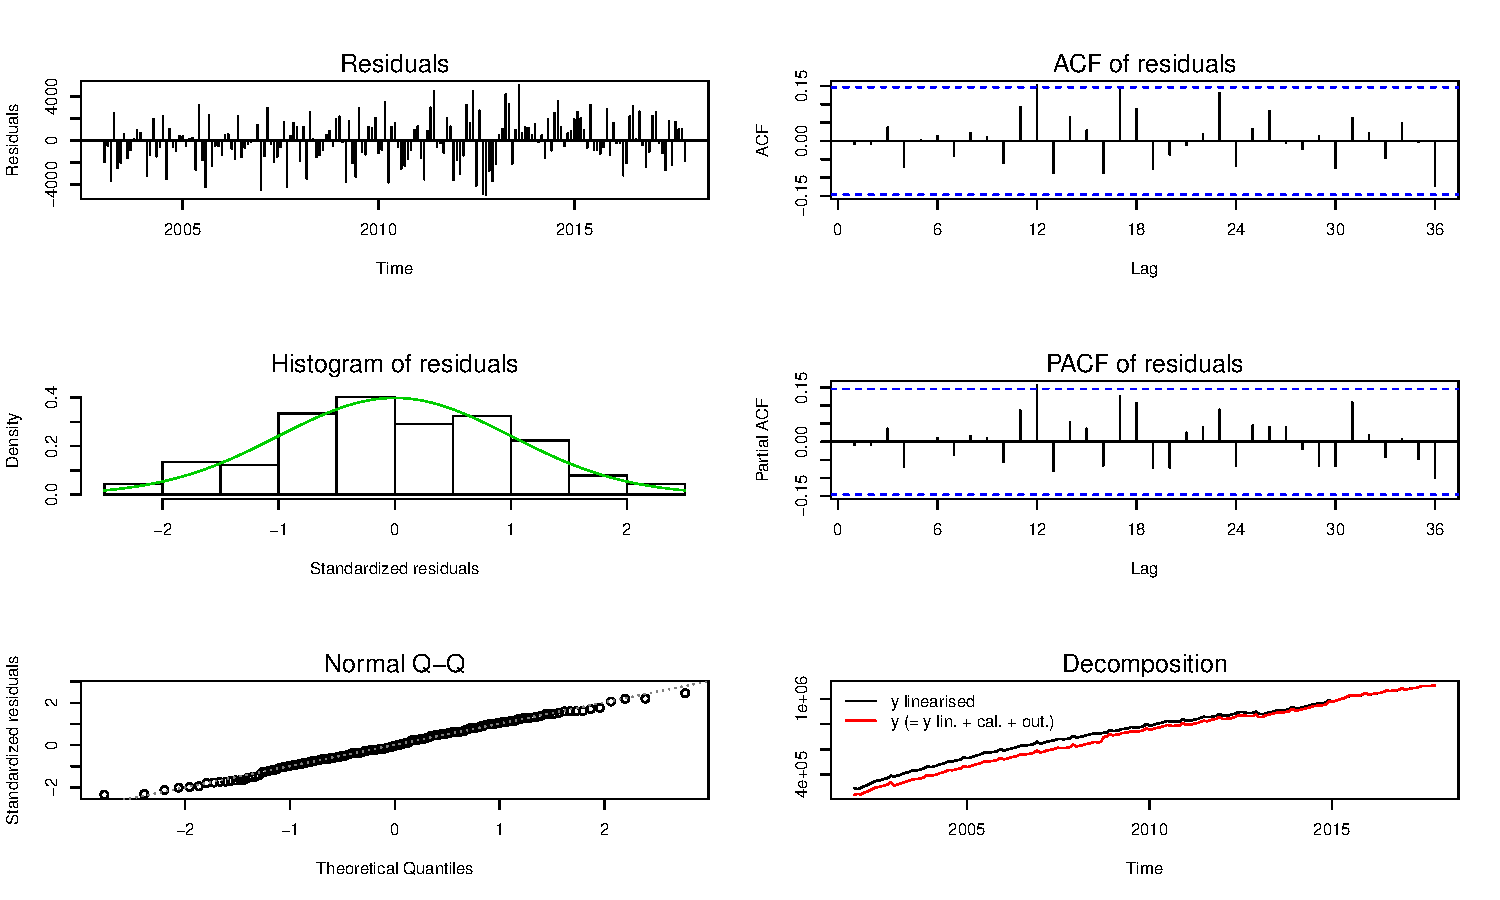
\includegraphics{rjdemetra_files/figure-beamer/unnamed-chunk-3-1.pdf}

\end{frame}

\begin{frame}[fragile]{RegARIMA examples (3/3)}

\footnotesize

To select a specific graph \texttt{which} parameter; \texttt{dec\_zoom}
for an additional regarima decomposition graph:

\begin{Shaded}
\begin{Highlighting}[]
\KeywordTok{plot}\NormalTok{(regarima_model, }\DataTypeTok{which =} \DecValTok{6}\NormalTok{, }\DataTypeTok{dec_zoom =} \OtherTok{TRUE}\NormalTok{)}
\end{Highlighting}
\end{Shaded}

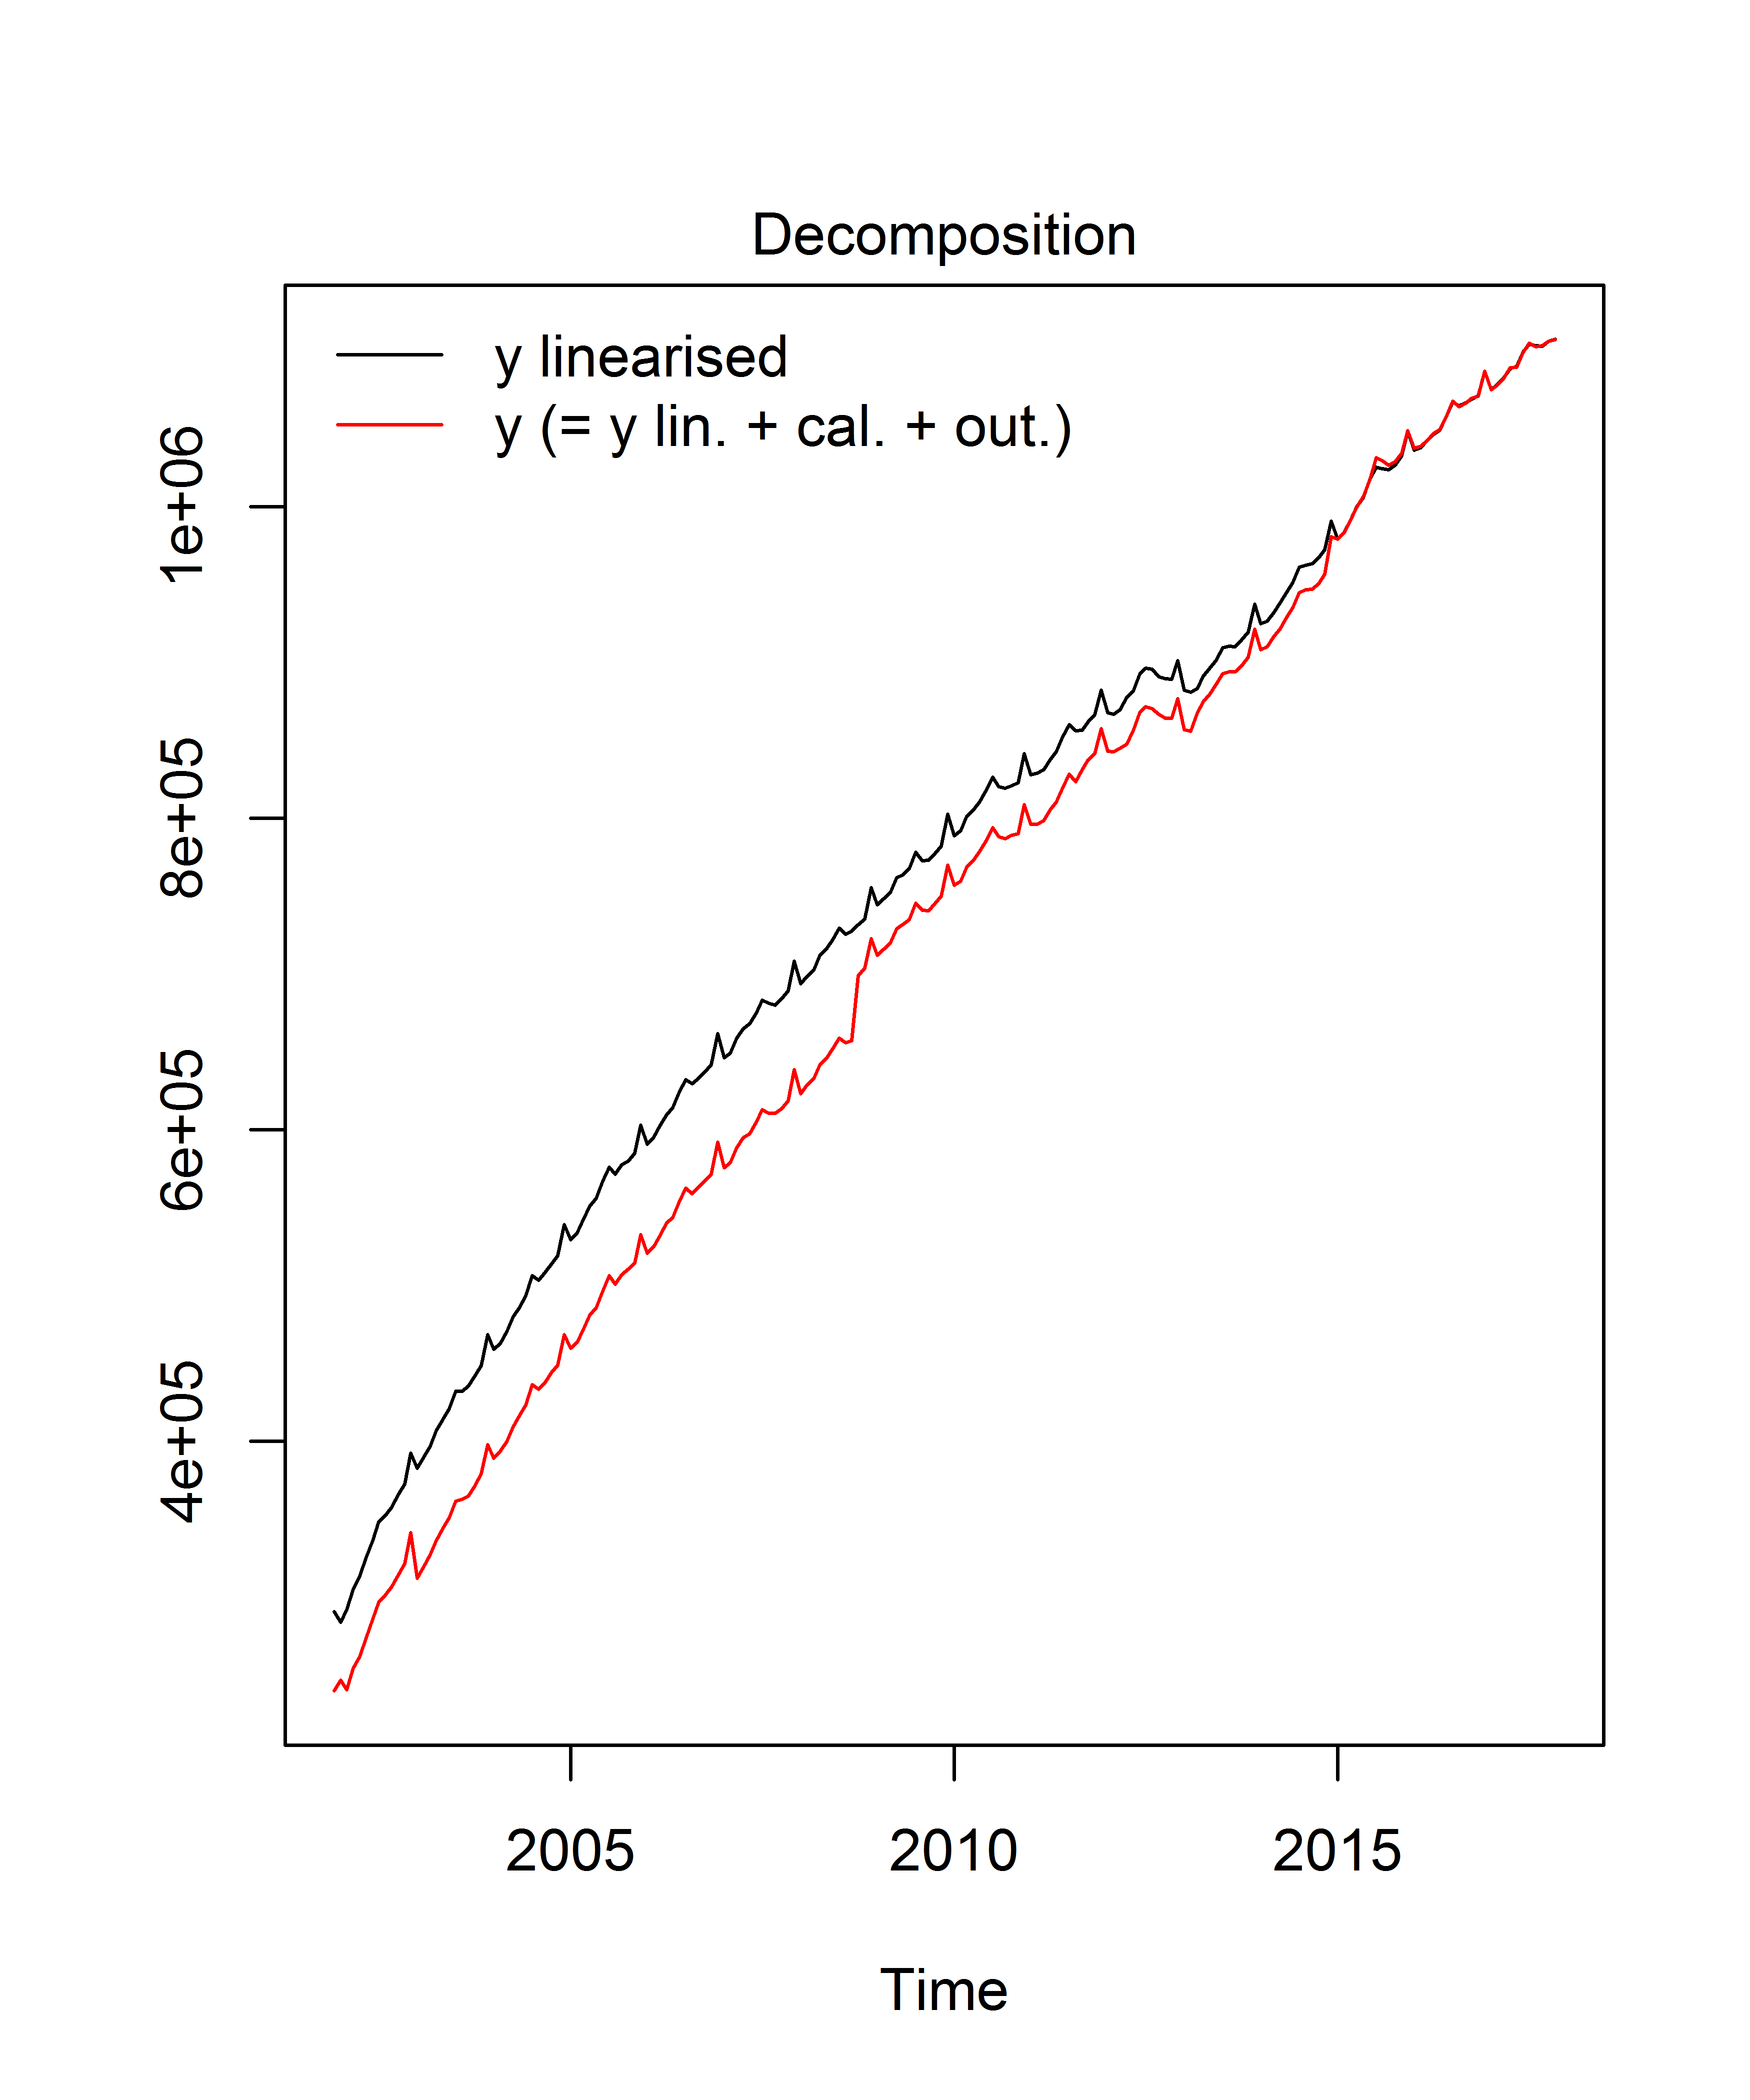
\includegraphics[width=0.4\paperwidth,height = 1.2\textheight]{img/regarima1.png}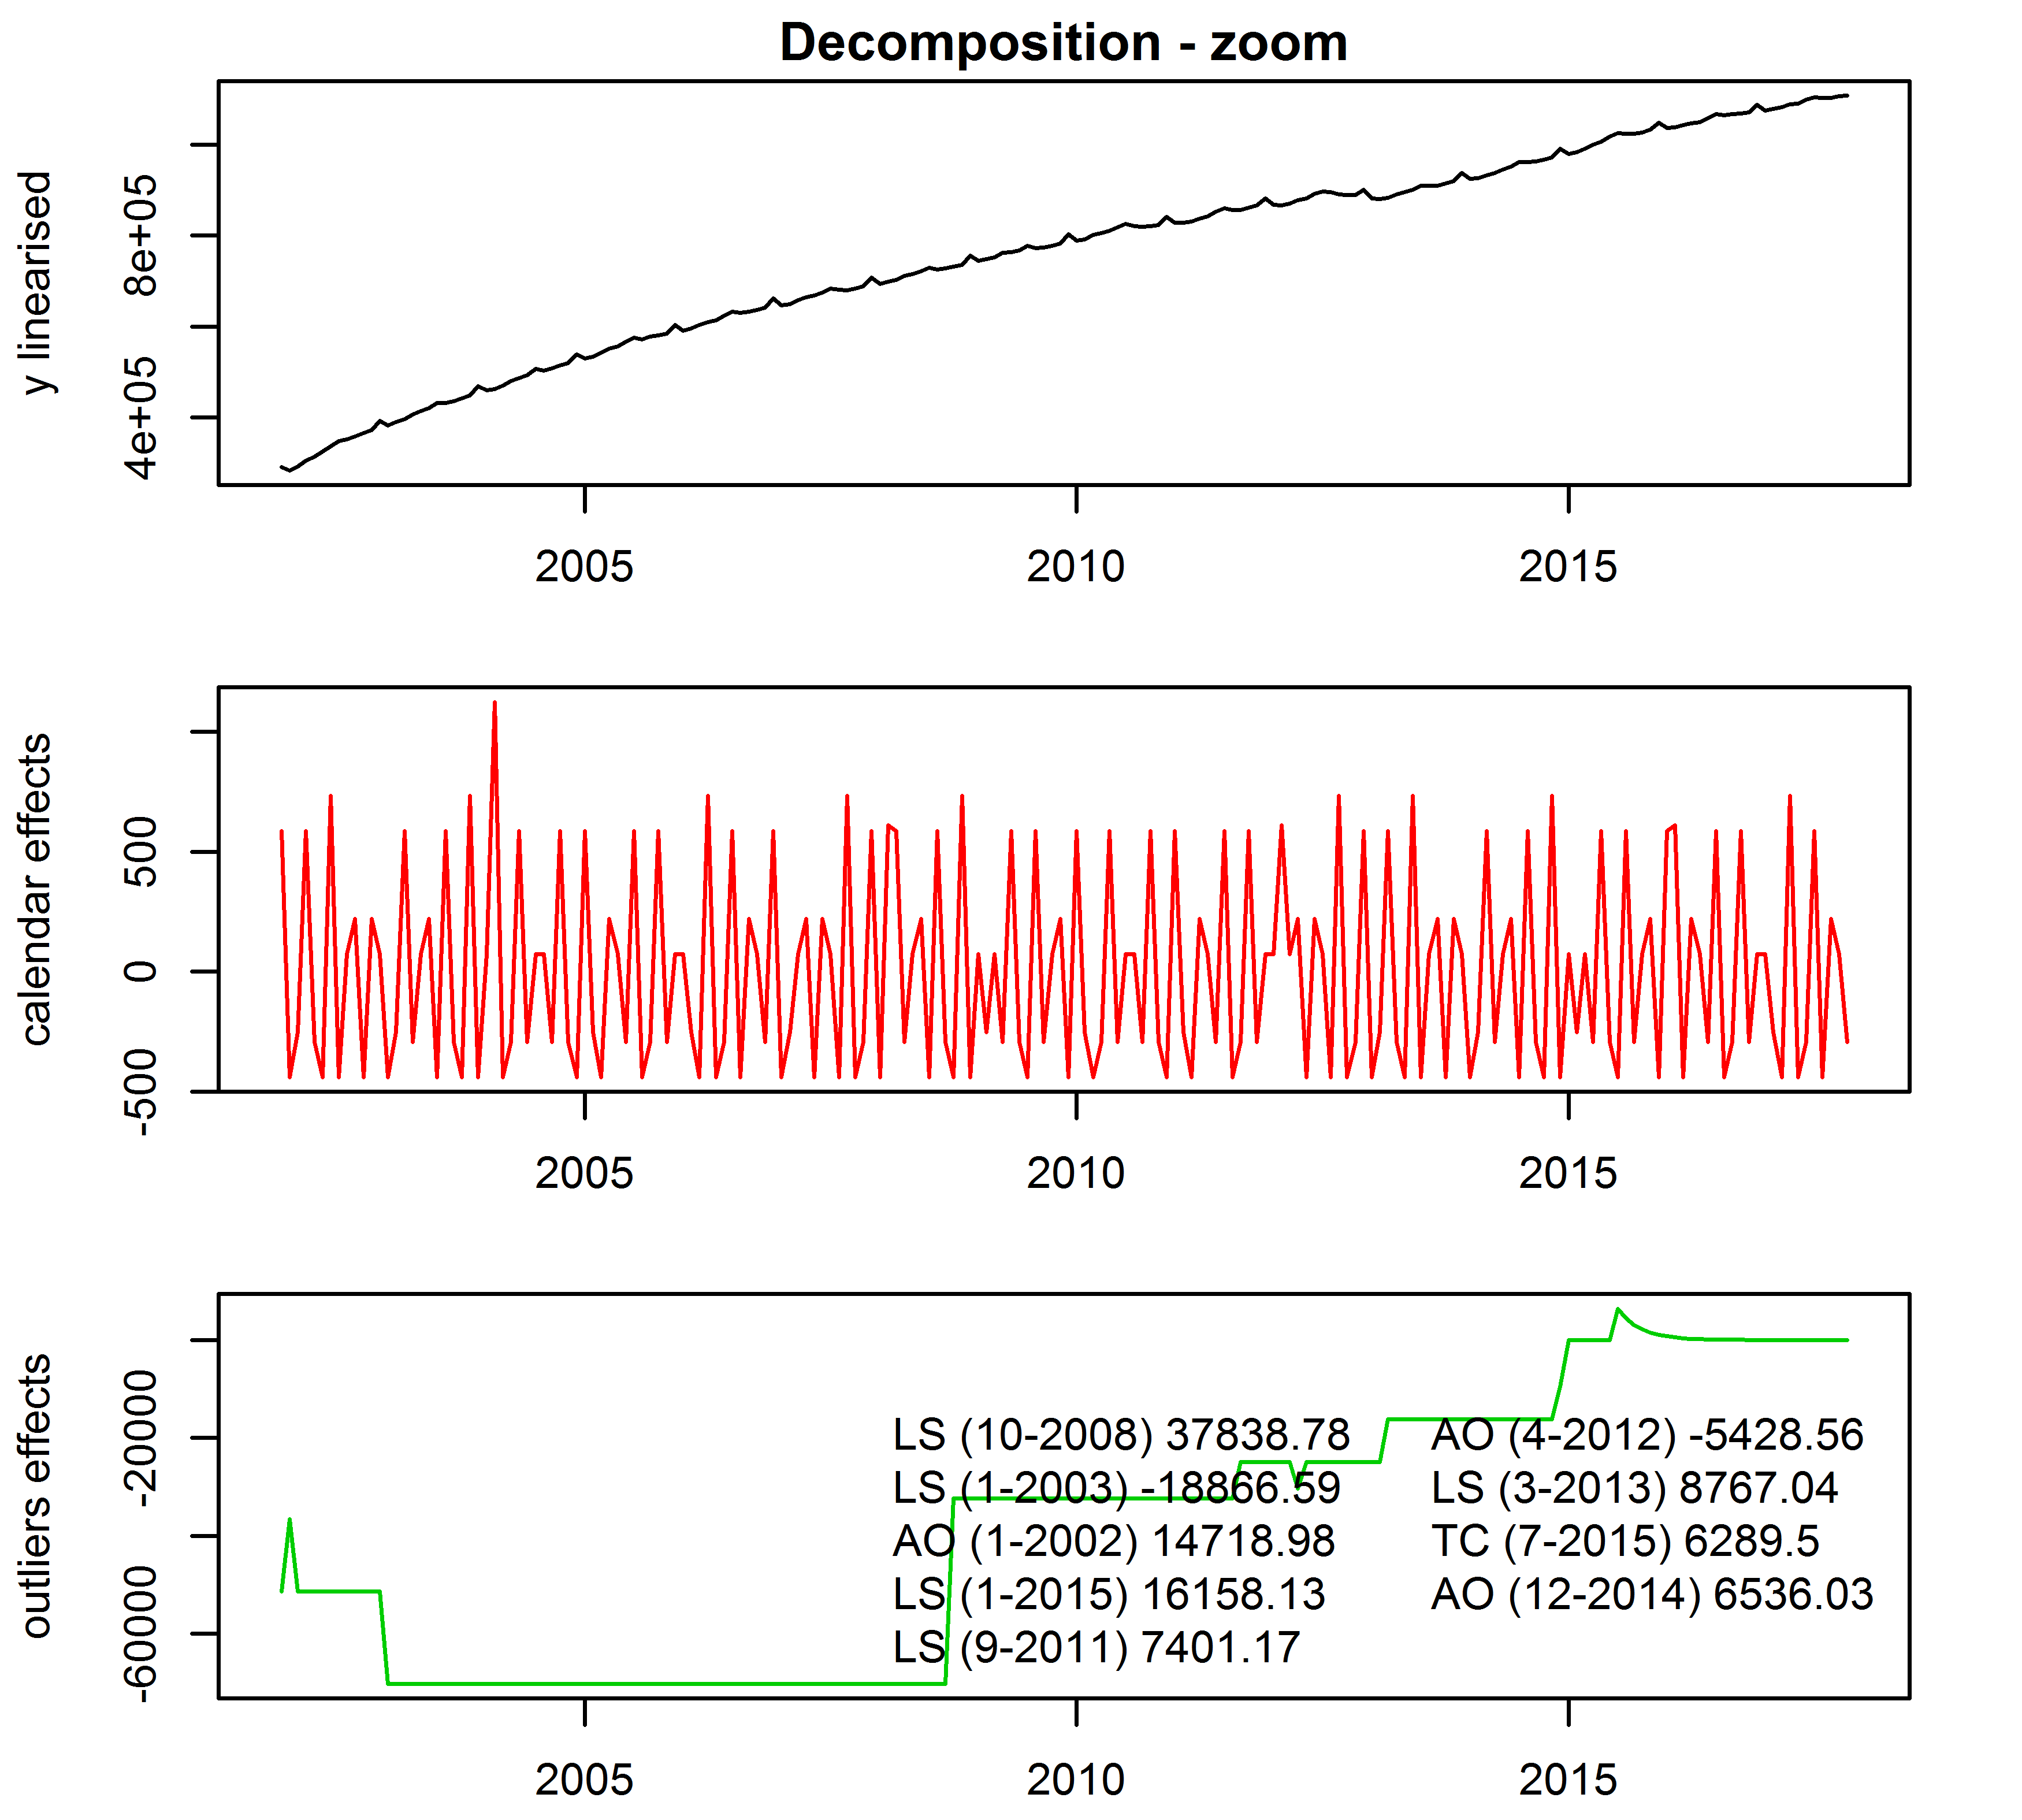
\includegraphics[width=0.5\paperwidth]{img/regarima2.png}

\end{frame}

\subsection{Seasonal adjustment
examples}\label{seasonal-adjustment-examples}

\begin{frame}[fragile]{Seasonal adjustment examples (1/7)}

A \texttt{SA} object is a \texttt{list()} of 5 elements:

\begin{enumerate}
\def\labelenumi{\arabic{enumi}.}
\tightlist
\item
  \texttt{regarima}: the RegArima model
\item
  \texttt{decomposition}: decomposition variables (\(\ne\) for
  TRAMO-SEATS and X-13-ARIMA)
\item
  \texttt{final}: time series main results
\item
  \texttt{diagnostics}: residuals tests, etc.
\item
  \texttt{user\_defined}: other user\_defined variables not exported by
  default (see \texttt{?user\_defined\_variables})
\end{enumerate}

\footnotesize

\begin{Shaded}
\begin{Highlighting}[]
\NormalTok{x13_usr_spec <-}\StringTok{ }\KeywordTok{x13_spec_def}\NormalTok{(}\DataTypeTok{spec=}\KeywordTok{c}\NormalTok{(}\StringTok{"RSA5c"}\NormalTok{),}\DataTypeTok{usrdef.outliersEnabled =} \OtherTok{TRUE}\NormalTok{,}
                             \DataTypeTok{usrdef.outliersType =} \KeywordTok{c}\NormalTok{(}\StringTok{"LS"}\NormalTok{,}\StringTok{"AO"}\NormalTok{),}
                             \DataTypeTok{usrdef.outliersDate=}\KeywordTok{c}\NormalTok{(}\StringTok{"2008-10-01"}\NormalTok{,}\StringTok{"2002-01-01"}\NormalTok{),}
                             \DataTypeTok{usrdef.outliersCoef =} \KeywordTok{c}\NormalTok{(}\DecValTok{36000}\NormalTok{,}\DecValTok{14000}\NormalTok{),}
                             \DataTypeTok{transform.function =} \StringTok{"None"}\NormalTok{)}
\NormalTok{x13_mod <-}\StringTok{ }\KeywordTok{x13}\NormalTok{(myseries, x13_usr_spec)}
\NormalTok{ts_mod <-}\StringTok{ }\KeywordTok{tramoseats_def}\NormalTok{(myseries, }\DataTypeTok{spec =} \StringTok{"RSAfull"}\NormalTok{)}
\end{Highlighting}
\end{Shaded}

\end{frame}

\begin{frame}[fragile]{Seasonal adjustment examples (2/7)}

\footnotesize

\begin{Shaded}
\begin{Highlighting}[]
\NormalTok{x13_mod}\OperatorTok{$}\NormalTok{decomposition}
\end{Highlighting}
\end{Shaded}

\begin{verbatim}
## Monitoring and Quality Assessment Statistics: 
##       M stats
## M(1)    0.026
## M(2)    0.011
## M(3)    0.000
## M(4)    0.423
## M(5)    0.000
## M(6)    0.095
## M(7)    0.188
## M(8)    0.356
## M(9)    0.128
## M(10)   0.385
## Q       0.144
## Q-M2    0.160
## 
## Final filters: 
## Seasonal filter:  3x5
## Trend filter:  9-Henderson
\end{verbatim}

\end{frame}

\begin{frame}[fragile]{Seasonal adjustment examples (3/7)}

\footnotesize

\begin{Shaded}
\begin{Highlighting}[]
\KeywordTok{print}\NormalTok{(ts_mod}\OperatorTok{$}\NormalTok{diagnostics, }\DataTypeTok{enable_print_style =} \OtherTok{FALSE}\NormalTok{)}
\end{Highlighting}
\end{Shaded}

\begin{verbatim}
##  Relative contribution of the components to the stationary portion of the variance in the original series, after the removal of the long term trend 
##  Trend computed by Hodrick-Prescott filter (cycle length = 8.0 years)
##            Component
##  Cycle        12.127
##  Seasonal      4.002
##  Irregular     0.000
##  TD & Hol.     0.000
##  Others       95.857
##  Total       111.986
## 
##  Residual seasonality tests 
##                                       P.value
##  qs test on sa                          1.000
##  qs test on i                           1.000
##  f-test on sa (seasonal dummies)        1.000
##  f-test on i (seasonal dummies)         0.998
##  Residual seasonality (entire series)   1.000
##  Residual seasonality (last 3 years)    0.998
##  f-test on sa (td)                      0.995
##  f-test on i (td)                       0.823
## 
##  Combined test in the entire series 
##  Non parametric tests for stable seasonality
##                                                           P.value
##    Kruskall-Wallis test                                      0.000
##    Test for the presence of seasonality assuming stability   0.000
##    Evolutive seasonality test                                0.151
##  
##  Identifiable seasonality present
## 
##  Combined test in the last 3 years 
##  Non parametric tests for stable seasonality
##                                                           P.value
##    Kruskall-Wallis test                                      0.001
##    Test for the presence of seasonality assuming stability   0.000
##    Evolutive seasonality test                                0.662
##  
##  Identifiable seasonality present
\end{verbatim}

\end{frame}

\begin{frame}[fragile]{Seasonal adjustment examples (4/7)}

\begin{Shaded}
\begin{Highlighting}[]
\KeywordTok{plot}\NormalTok{(x13_mod}\OperatorTok{$}\NormalTok{decomposition)}
\end{Highlighting}
\end{Shaded}

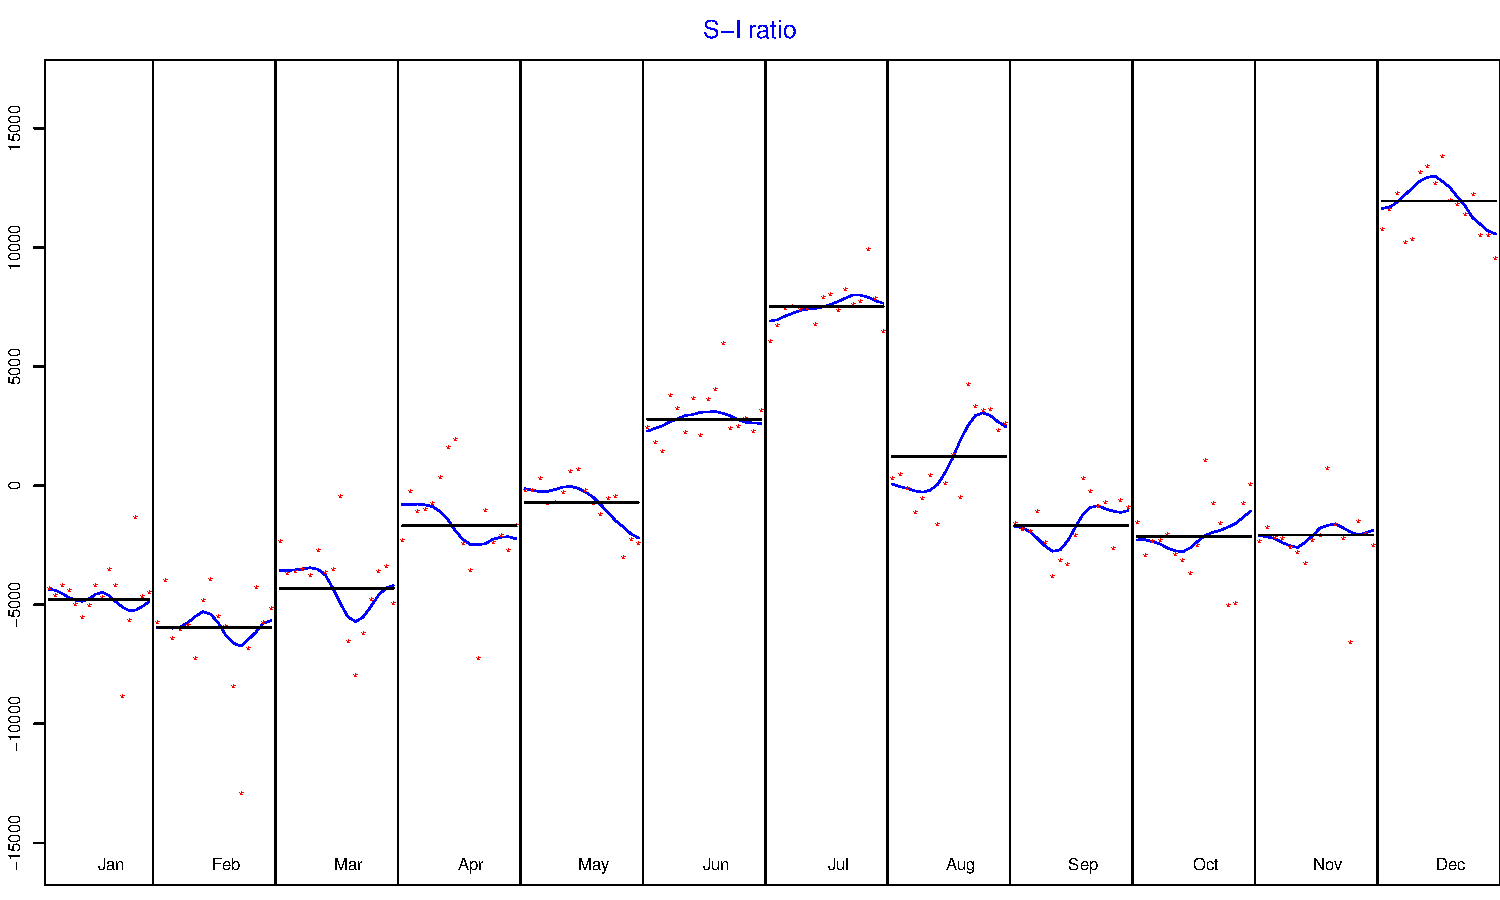
\includegraphics{rjdemetra_files/figure-beamer/unnamed-chunk-9-1.pdf}

\end{frame}

\begin{frame}[fragile]{Seasonal adjustment examples (5/7)}

\footnotesize

\begin{Shaded}
\begin{Highlighting}[]
\NormalTok{x13_mod}\OperatorTok{$}\NormalTok{final}
\end{Highlighting}
\end{Shaded}

\begin{verbatim}
## Last observed values
##                y      sa       t          s           i
## Dec 2016 1087082 1075842 1076809 11240.0563  -966.92838
## Jan 2017 1075137 1080586 1080172 -5448.7173   413.95902
## Feb 2017 1078141 1084192 1083675 -6050.8123   516.52696
## Mar 2017 1082422 1086339 1087148 -3917.3376  -808.74611
## Apr 2017 1089204 1090829 1090257 -1625.1053   571.84127
## May 2017 1089662 1092839 1092962 -3177.2306  -122.51812
## Jun 2017 1099145 1096159 1095433  2985.8807   726.30641
## Jul 2017 1104797 1096917 1097978  7880.4569 -1061.84552
## Aug 2017 1102805 1100832 1100754  1972.7310    78.66638
## Sep 2017 1103295 1103768 1103873  -473.3715  -104.16916
## Oct 2017 1106170 1107814 1107030 -1643.7937   783.96096
## Nov 2017 1107118 1108997 1109863 -1879.3688  -865.76589
## 
## Forecasts:
##               y       sa        t          s           i
## Dec 2001 239720 227861.6 228866.4 11858.4223 -1004.78113
## Jan 2002 246680 251538.2 237528.5 -4858.1935 14009.64528
## Feb 2002 240476 246817.1 246601.3 -6341.1081   215.77338
## Mar 2002 254298 256967.3 255762.6 -2669.3308  1204.75400
## Apr 2002 261655 263341.0 264796.1 -1685.9858 -1455.07022
## May 2002 273847 273692.9 273676.1   154.0887    16.80276
## Jun 2002 285696 282806.5 282533.3  2889.5090   273.22470
## Jul 2002 296574 290653.5 291405.6  5920.5102  -752.06256
## Aug 2002 301114 300386.3 300115.3   727.7317   270.97891
## Sep 2002 306676 308469.8 308401.1 -1793.8464    68.72927
## Oct 2002 313872 316654.3 316081.5 -2782.3279   572.85709
## Nov 2002 321353 322878.9 323254.1 -1525.9499  -375.12371
\end{verbatim}

\end{frame}

\begin{frame}[fragile]{Seasonal adjustment examples (6/7)}

\begin{Shaded}
\begin{Highlighting}[]
\KeywordTok{plot}\NormalTok{(x13_mod}\OperatorTok{$}\NormalTok{final, }\DataTypeTok{first_date =} \DecValTok{2012}\NormalTok{, }\DataTypeTok{type_chart =} \StringTok{"sa-trend"}\NormalTok{)}
\end{Highlighting}
\end{Shaded}

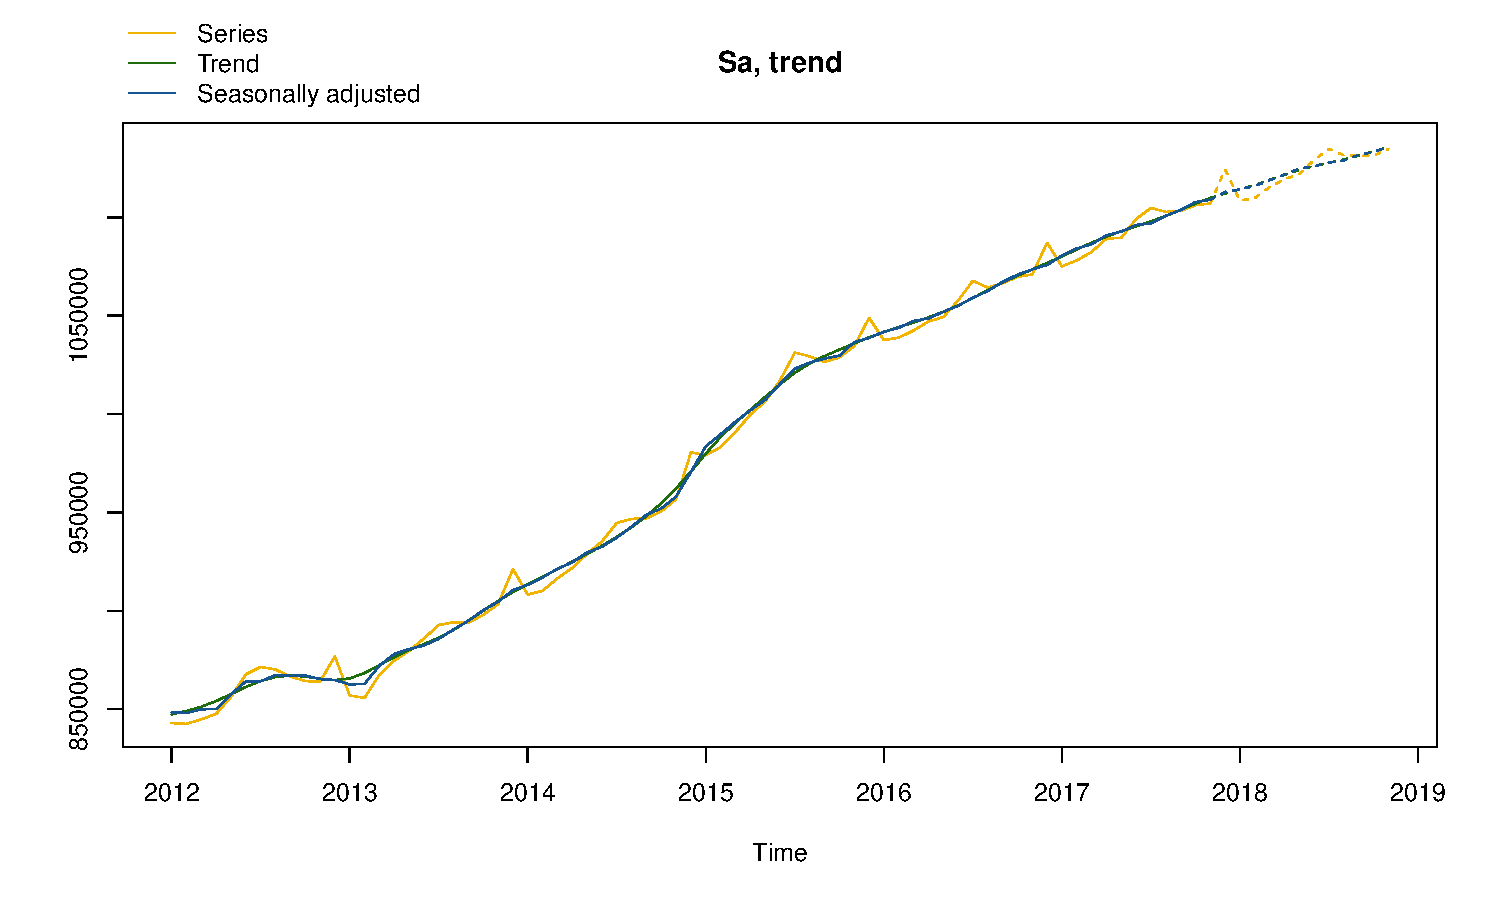
\includegraphics{rjdemetra_files/figure-beamer/unnamed-chunk-11-1.pdf}

\end{frame}

\begin{frame}[fragile]{Seasonal adjustment examples (7/7)}

\footnotesize

\begin{Shaded}
\begin{Highlighting}[]
\KeywordTok{print}\NormalTok{(x13_mod}\OperatorTok{$}\NormalTok{diagnostics, }\DataTypeTok{enable_print_style =} \OtherTok{FALSE}\NormalTok{)}
\end{Highlighting}
\end{Shaded}

\begin{verbatim}
##  Relative contribution of the components to the stationary portion of the variance in the original series, after the removal of the long term trend 
##  Trend computed by Hodrick-Prescott filter (cycle length = 8.0 years)
##            Component
##  Cycle        27.110
##  Seasonal      7.795
##  Irregular     0.382
##  TD & Hol.     0.114
##  Others       87.839
##  Total       123.240
## 
##  Residual seasonality tests 
##                                       P.value
##  qs test on sa                          1.000
##  qs test on i                           1.000
##  f-test on sa (seasonal dummies)        0.967
##  f-test on i (seasonal dummies)         0.854
##  Residual seasonality (entire series)   0.967
##  Residual seasonality (last 3 years)    0.967
##  f-test on sa (td)                      0.878
##  f-test on i (td)                       0.734
## 
##  Combined test in the entire series 
##  Non parametric tests for stable seasonality
##                                                           P.value
##    Kruskall-Wallis test                                      0.000
##    Test for the presence of seasonality assuming stability   0.000
##    Evolutive seasonality test                                0.032
##  
##  Identifiable seasonality present
## 
##  Combined test in the last 3 years 
##  Non parametric tests for stable seasonality
##                                                           P.value
##    Kruskall-Wallis test                                      0.002
##    Test for the presence of seasonality assuming stability   0.000
##    Evolutive seasonality test                                0.404
##  
##  Identifiable seasonality probably present
\end{verbatim}

\end{frame}

\subsection{Manipulate workspaces}\label{manipulate-workspaces}

\begin{frame}[fragile]{Export a workspace}

\footnotesize

\begin{Shaded}
\begin{Highlighting}[]
\NormalTok{wk <-}\StringTok{ }\KeywordTok{new_workspace}\NormalTok{()}
\KeywordTok{new_multiprocessing}\NormalTok{(wk, }\StringTok{"sa1"}\NormalTok{)}
\KeywordTok{add_sa_item}\NormalTok{(wk, }\DataTypeTok{multiprocessing =} \StringTok{"sa1"}\NormalTok{,}
\NormalTok{            x13_mod)}
\KeywordTok{add_sa_item}\NormalTok{(wk, }\DataTypeTok{multiprocessing =} \StringTok{"sa1"}\NormalTok{,}
\NormalTok{            ts_mod, }\StringTok{"TramoSeats"}\NormalTok{)}
\KeywordTok{save_workspace}\NormalTok{(wk, }\StringTok{"workspace.xml"}\NormalTok{)}
\end{Highlighting}
\end{Shaded}

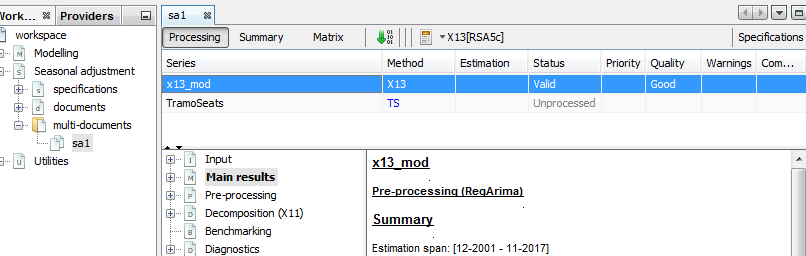
\includegraphics{img/workspace.png}

\end{frame}

\begin{frame}[fragile]{Import a workspace (1/3)}

\footnotesize

\begin{Shaded}
\begin{Highlighting}[]
\NormalTok{wk <-}\StringTok{ }\KeywordTok{load_workspace}\NormalTok{(}\StringTok{"workspace.xml"}\NormalTok{)}
\KeywordTok{get_ts}\NormalTok{(wk)}
\end{Highlighting}
\end{Shaded}

\begin{verbatim}
## $sa1
## $sa1$x13_mod
##          Jan     Feb     Mar     Apr     May     Jun     Jul     Aug
## 2001                                                                
## 2002  246680  240476  254298  261655  273847  285696  296574  301114
## 2003  312120  319317  327218  336320  343756  351042  361475  362668
## 2004  389117  393469  399591  409373  416623  423014  436246  433400
## 2005  459893  463566  471751  481074  485829  496407  506284  500775
## 2006  520777  524765  532187  540257  543523  553658  562621  558909
## 2007  575640  578720  588522  594796  597610  604978  612926  610644
## 2008  623127  628987  632868  641391  645746  652087  658817  655993
## 2009  712199  715829  719841  729136  731911  734897  745341  741044
## 2010  757084  759517  768585  772608  778963  785493  793930  787969
## 2011  796249  796244  798344  805450  810435  819663  828194  823445
## 2012  842958  842541  844906  847598  856303  867744  871509  870166
## 2013  856975  855786  867536  874708  879698  885908  892804  894196
## 2014  908272  910194  916522  921814  928897  935294  944707  946755
## 2015  979087  983220  990949  999766 1006424 1017083 1031285 1029364
## 2016 1037667 1038867 1042518 1047084 1049349 1057708 1067801 1064305
## 2017 1075137 1078141 1082422 1089204 1089662 1099145 1104797 1102805
##          Sep     Oct     Nov     Dec
## 2001                          239720
## 2002  306676  313872  321353  341158
## 2003  364830  371239  379148  397902
## 2004  438041  444394  448753  468426
## 2005  507014  510363  514338  532738
## 2006  563110  566998  571419  592122
## 2007  610479  613502  618655  638551
## 2008  657080  698784  703624  722746
## 2009  740515  745290  749965  769871
## 2010  786756  789040  790206  808562
## 2011  831170  837498  841367  857482
## 2012  866652  864266  864074  876787
## 2013  894026  897951  903364  921221
## 2014  947025  950566  956813  980634
## 2015 1026546 1028789 1034492 1048926
## 2016 1066501 1069742 1070979 1087082
## 2017 1103295 1106170 1107118        
## 
## $sa1$TramoSeats
##          Jan     Feb     Mar     Apr     May     Jun     Jul     Aug
## 2001                                                                
## 2002  246680  240476  254298  261655  273847  285696  296574  301114
## 2003  312120  319317  327218  336320  343756  351042  361475  362668
## 2004  389117  393469  399591  409373  416623  423014  436246  433400
## 2005  459893  463566  471751  481074  485829  496407  506284  500775
## 2006  520777  524765  532187  540257  543523  553658  562621  558909
## 2007  575640  578720  588522  594796  597610  604978  612926  610644
## 2008  623127  628987  632868  641391  645746  652087  658817  655993
## 2009  712199  715829  719841  729136  731911  734897  745341  741044
## 2010  757084  759517  768585  772608  778963  785493  793930  787969
## 2011  796249  796244  798344  805450  810435  819663  828194  823445
## 2012  842958  842541  844906  847598  856303  867744  871509  870166
## 2013  856975  855786  867536  874708  879698  885908  892804  894196
## 2014  908272  910194  916522  921814  928897  935294  944707  946755
## 2015  979087  983220  990949  999766 1006424 1017083 1031285 1029364
## 2016 1037667 1038867 1042518 1047084 1049349 1057708 1067801 1064305
## 2017 1075137 1078141 1082422 1089204 1089662 1099145 1104797 1102805
##          Sep     Oct     Nov     Dec
## 2001                          239720
## 2002  306676  313872  321353  341158
## 2003  364830  371239  379148  397902
## 2004  438041  444394  448753  468426
## 2005  507014  510363  514338  532738
## 2006  563110  566998  571419  592122
## 2007  610479  613502  618655  638551
## 2008  657080  698784  703624  722746
## 2009  740515  745290  749965  769871
## 2010  786756  789040  790206  808562
## 2011  831170  837498  841367  857482
## 2012  866652  864266  864074  876787
## 2013  894026  897951  903364  921221
## 2014  947025  950566  956813  980634
## 2015 1026546 1028789 1034492 1048926
## 2016 1066501 1069742 1070979 1087082
## 2017 1103295 1106170 1107118
\end{verbatim}

\end{frame}

\begin{frame}[fragile]{Import a workspace (2/3)}

\footnotesize

\begin{Shaded}
\begin{Highlighting}[]
\KeywordTok{compute}\NormalTok{(wk) }\CommentTok{# Important to get the Sa model}
\NormalTok{models <-}\StringTok{ }\KeywordTok{get_model}\NormalTok{(wk) }\CommentTok{# A progress bar is printed by default}
\end{Highlighting}
\end{Shaded}

\begin{verbatim}
## Multiprocessing 1 on 1:
## 
  |                                                                       
  |                                                                 |   0%
  |                                                                       
  |================================                                 |  50%
  |                                                                       
  |=================================================================| 100%
\end{verbatim}

\begin{Shaded}
\begin{Highlighting}[]
\CommentTok{# To extract only one model}
\NormalTok{mp <-}\StringTok{ }\KeywordTok{get_object}\NormalTok{(wk, }\DecValTok{1}\NormalTok{)}
\KeywordTok{count}\NormalTok{(mp)}
\end{Highlighting}
\end{Shaded}

\begin{verbatim}
## [1] 2
\end{verbatim}

\begin{Shaded}
\begin{Highlighting}[]
\NormalTok{sa2 <-}\StringTok{ }\KeywordTok{get_object}\NormalTok{(mp,}\DecValTok{2}\NormalTok{)}
\KeywordTok{get_name}\NormalTok{(sa2)}
\end{Highlighting}
\end{Shaded}

\begin{verbatim}
## [1] "TramoSeats"
\end{verbatim}

\begin{Shaded}
\begin{Highlighting}[]
\NormalTok{mod <-}\StringTok{ }\KeywordTok{get_model}\NormalTok{(wk, sa2)}
\end{Highlighting}
\end{Shaded}

\begin{verbatim}
## Multiprocessing 1 on 1:
## 
  |                                                                       
  |                                                                 |   0%
  |                                                                       
  |================================                                 |  50%
  |                                                                       
  |=================================================================| 100%
\end{verbatim}

\end{frame}

\begin{frame}{Import a workspace (3/3)}

\bcsmmh Still some bugs importing a workspace created by JDemetra+ when:

\begin{itemize}
\item
  The workspace contains user-defined trading days regressors
\item
  The workspace contains an invalid model
\end{itemize}

\end{frame}

\subsection{How to install and contribute to the
package?}\label{how-to-install-and-contribute-to-the-package}

\begin{frame}[fragile]{How to install the package?}

The package is available on github:
\url{https://github.com/nbbrd/rjdemetra}

\bcinfo To install it you need Java8: in case you don't, install a
portable version of Java8 and set the \texttt{JAVA\_HOME} path.

To install it use \texttt{devtools} or download the zip file

\begin{Shaded}
\begin{Highlighting}[]
\CommentTok{# install.packages("devtools")}
\NormalTok{devtools}\OperatorTok{::}\KeywordTok{install_github}\NormalTok{(}\StringTok{"nbbrd/rjdemetra"}\NormalTok{,}
                         \DataTypeTok{args =} \StringTok{"--no-multiarch"}\NormalTok{)}
\end{Highlighting}
\end{Shaded}

\end{frame}

\begin{frame}{How to contribute to the package?}

You can contribute:

\begin{itemize}
\item
  Testing it and reporting issues
  (\url{https://github.com/nbbrd/rjdemetra/issues})
\item
  Correcting issues (\url{https://github.com/nbbrd/rjdemetra/pulls})
\item
  Developping new tools (other packages, new functions, etc.)
\end{itemize}

\end{frame}

\subsection{Future developments}\label{future-developments}

\begin{frame}[fragile]{What's next? \bcpanchant}

\begin{itemize}
\item
  Possibility to used user-defined calendar regressors
\item
  \texttt{update} function to refresh a model with new data
\item
  Include a ``complete'' dataset in the package
\item
  Write a vignette (long-form guide to the package)
\item
  More tests on the package
\end{itemize}

\end{frame}

\section{One addin example: rdjqa}\label{one-addin-example-rdjqa}

\subsection{What for?}\label{what-for}

\begin{frame}[fragile]{What for?}

A package for quality assessment for seasonal adjustment. It implements:

\begin{itemize}
\item
  Statistics Canada Dashboard (to provide a snapshot of an individual
  series at a point in time and points out some possible problems)
\item
  Insee quality report matrix (used to help the analyst during
  production to prioritize the models to check)
\end{itemize}

\(\rightarrow\) See the
\href{https://ec.europa.eu/eurostat/web/products-manuals-and-guidelines/-/KS-GQ-18-001?inheritRedirect=true}{Seasonal
Adjustment handbook}

Available on github \url{https://github.com/AQLT/rjdqa}, still in
development (only works for X13 models and no documentation yet)

Example of the dashboard:

\begin{Shaded}
\begin{Highlighting}[]
\KeywordTok{library}\NormalTok{(rjdqa)}
\KeywordTok{plot}\NormalTok{(}\KeywordTok{sa_dashboard}\NormalTok{(x13_mod))}
\end{Highlighting}
\end{Shaded}

\end{frame}

\subsection{Statistics Canada
dashboard}\label{statistics-canada-dashboard}

\begin{frame}{Example of the dashboard (1/2)}

\footnotesize
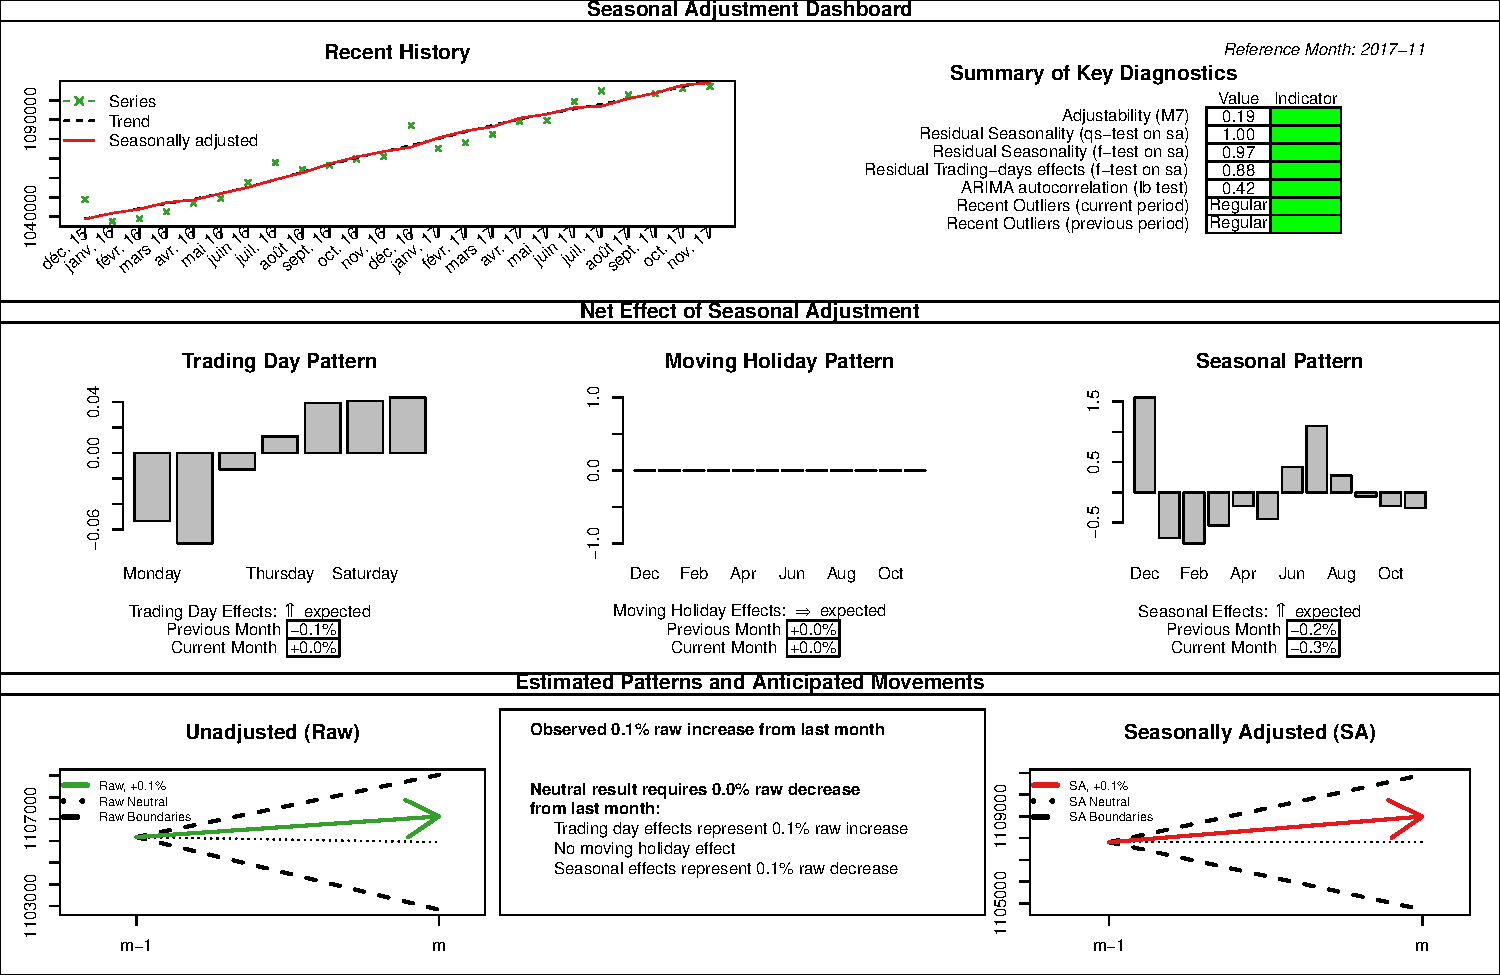
\includegraphics{rjdemetra_files/figure-beamer/unnamed-chunk-17-1.pdf}

\end{frame}

\begin{frame}{Example of the dashboard (2/2)}

\begin{enumerate}
\def\labelenumi{\arabic{enumi}.}
\item
  \textbf{Recent History of Series}: plot of the raw series, the SA
  series and the trend for the most recent periods. It is intended to
  identify trend direction, overall volatility and obvious outliers
\item
  \textbf{Summary of Key Diagnostics}: key diagnostics as residual
  seasonality, recent and recurring outliers, moving seasonality, ARIMA
  model autocorrelation
\item
  \textbf{Estimated Patterns and Anticipated Movements}: estimated
  trading day, moving holiday and seasonal pattern (rescaled in additive
  decomposition to represent relative level)
\item
  \textbf{Net Effect of Seasonal Adjustment}: movement in the raw
  series, compared to typical ranges centered around ``neutral'' value
  (when \(SA_t = SA_{t-1}\))
\end{enumerate}

\end{frame}

\end{document}
